% This is samplepaper.tex, a sample chapter demonstrating the
% LLNCS macro package for Springer Computer Science proceedings;
% Version 2.20 of 2017/10/04
%
\documentclass[runningheads]{llncs}
%
\usepackage{graphicx}
\usepackage{dirtytalk}
\usepackage{enumitem}
\usepackage{pifont}
\usepackage{float}

% \usepackage{floatflt}% package for floatingfigure environment

% Used for displaying a sample figure. If possible, figure files should
% be included in EPS format.
%
% If you use the hyperref package, please uncomment the following line
% to display URLs in blue roman font according to Springer's eBook style:
% \renewcommand\UrlFont{\color{blue}\rmfamily}

\begin{document}
% Welche Aufgaben hat unser System? Was brauchen wir für Komponenten zur Realisierung? Wie können wir die sinnvoll in Threads unterteilen?
\title{Progress Report: Chinese Whispers}

\author{Group 1: Nadine Bisswang (804957) \and Johannes Deufel (804958) \and Jonas Pfaff (804930) \and Philipp Straub (804934)}

\authorrunning{Group 1: Nadine Bisswang \and Johannes Deufel \and Jonas Pfaff \and Philipp Straub}

\institute{}
%
\maketitle              % typeset the header of the contribution
\section{Introduction}
    As part of the Distributed System Project, we would like to implement the game \say{chinese whispers} (german: \say{Stille Post}) in a distributed system as part of the examination performance. 
    This historical children's game primarily serves the perceptual education of children and is didactically very valuable especially at kindergarten age. The goal of the game is for all players involved to correctly pass on a previously selected word or phrase. The attraction of the game (for the kids and educators) results from the fact that the last player has to pronounce what has been passed on aloud - this often results in very funny misunderstandings. 
    
    In the computer-assisted version, additional points are introduced in order to be able to choose a winner at the end of the game round. Just like in kindergarten, it must also be possible for individual players to leave the circle. Furthermore, the game must continue if the game leaders (educators) have to move away from the group (or, in IT-terms: crash).
    
    It is very exciting to map this game within a distributed system, as it is also formed in reality from many, distributed players. Without the distribution or the participation of at least four players, the game is not playable. Furthermore, the system follows a synchronous approach, since - just like in the real game - you have to wait for the previous player to pass on what he understood.
    
\section{Project Design}

    \subsection{Project Structure}
    Currently we plan to develop the middleware on the one hand and the game-logic on the other hand. The middleware should make use of UDP and TCP sockets available in python to implement the functionalities of the distributed system and fulfill the three main requirements set for it. The game-logic should make use the of the communication abstraction and ensure the correct procedure. 
    
    \subsection{System Architecture}
    Chinese Whispers is a game with a de-central organization. All members are of the same kind with one leader who is responsible for one additional task. Therefore we decided to choose a Peer-to-Peer Network for the implementation. The following visualization of the system architecture in Figure \ref{fig:architecture} describes the system behaviour once the game has started and a game leader was elected.

    \begin{figure}
        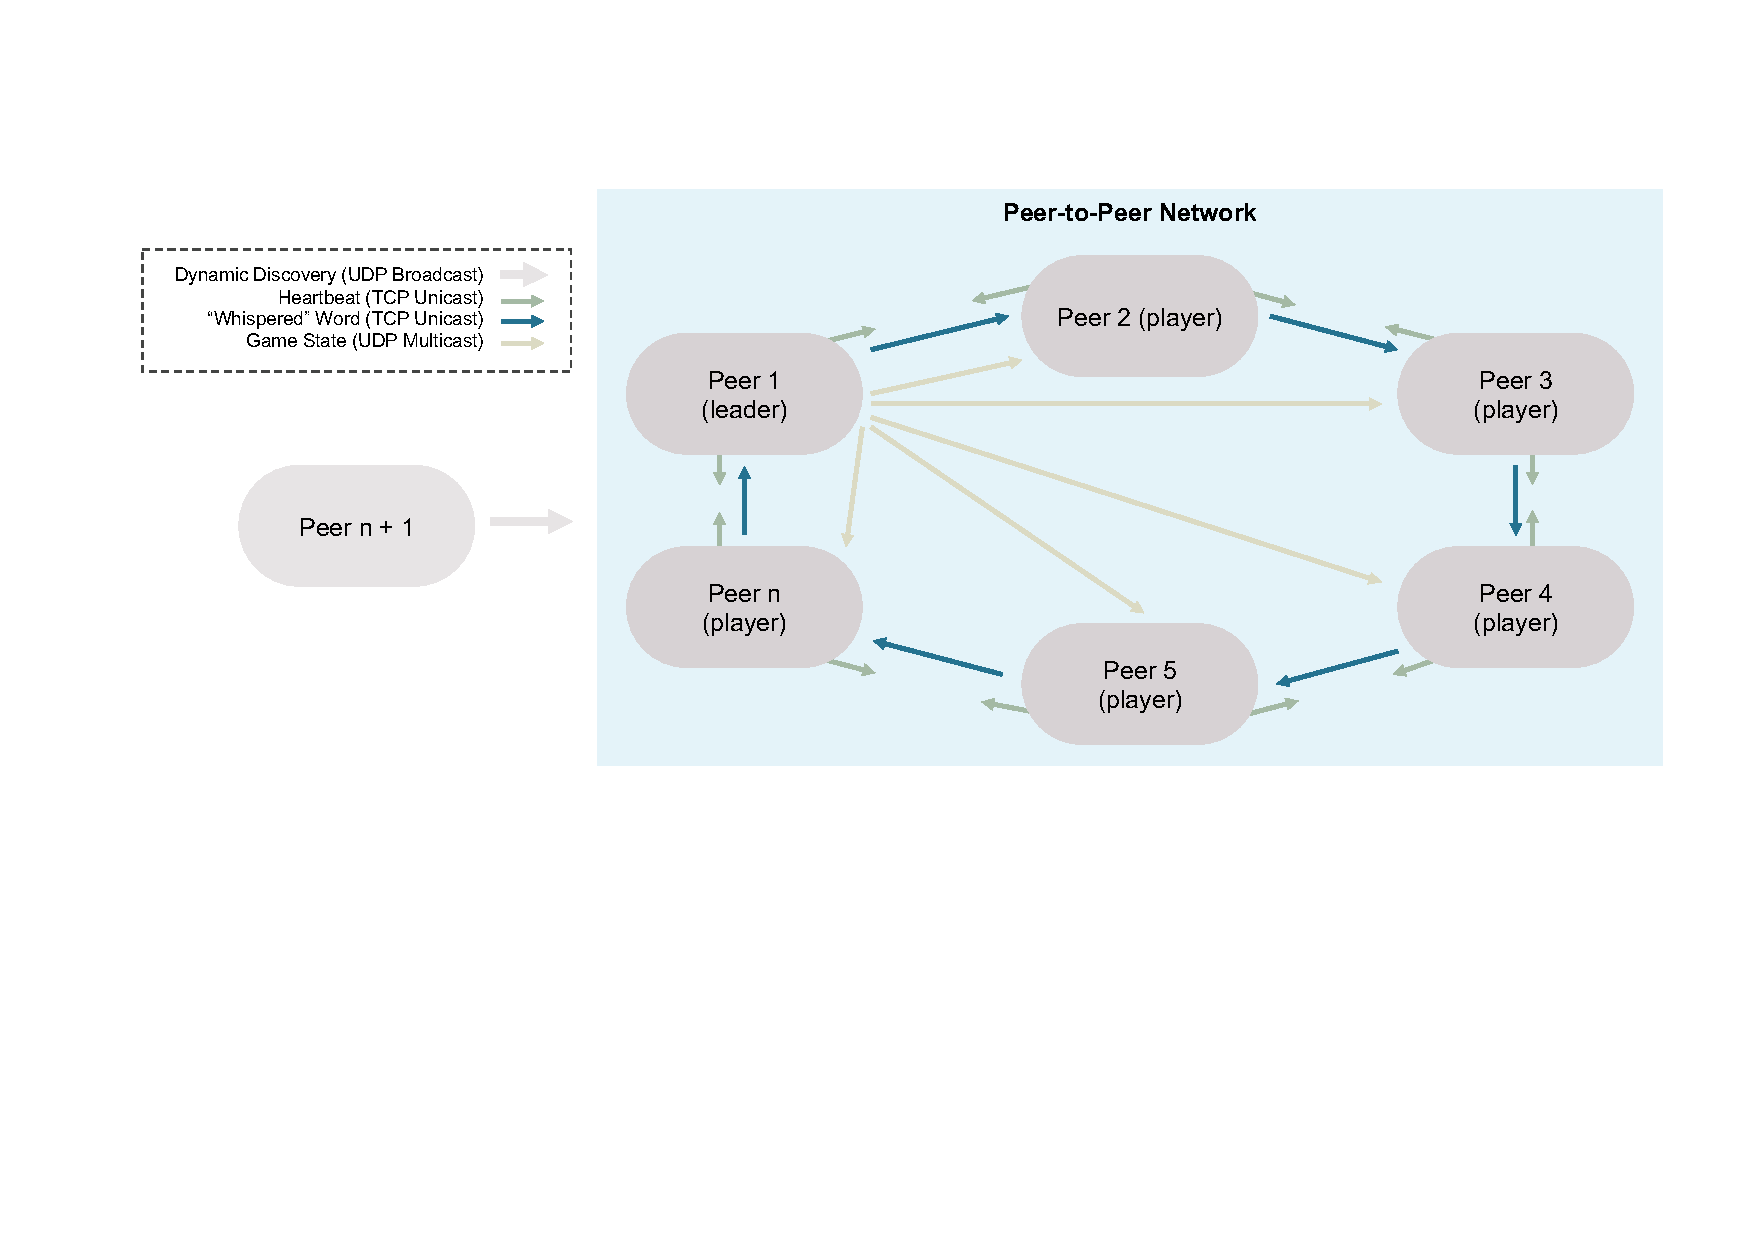
\includegraphics[width=\textwidth]{architecture.pdf}
        \caption{System Architecture} \label{fig:architecture}
    \end{figure}

\section{Project Requirements Implementation Plan}
    \subsection{Dynamic discovery of hosts}
        To enable our solution to be dynamically joined and left, we implement the dynamic discovery of hosts. For a Peer-to-Peer architecture we see different scenarios how dynamic discovery will appear: 
        
        - A peer starts and a network already exists, 
        
        - a peer starts and is the first node of a network or 
        
        - a peer is already a node in a network.
        
        In each of these cases, each peer creates, manages and shares its own group view. However, before any other task is done, each peer creates its own TCP unicast listener and a UDP broadcast listener that run in parallel with threading. This approach is illustrated in the Figure 2 below.
        
        \begin{figure}[H]
        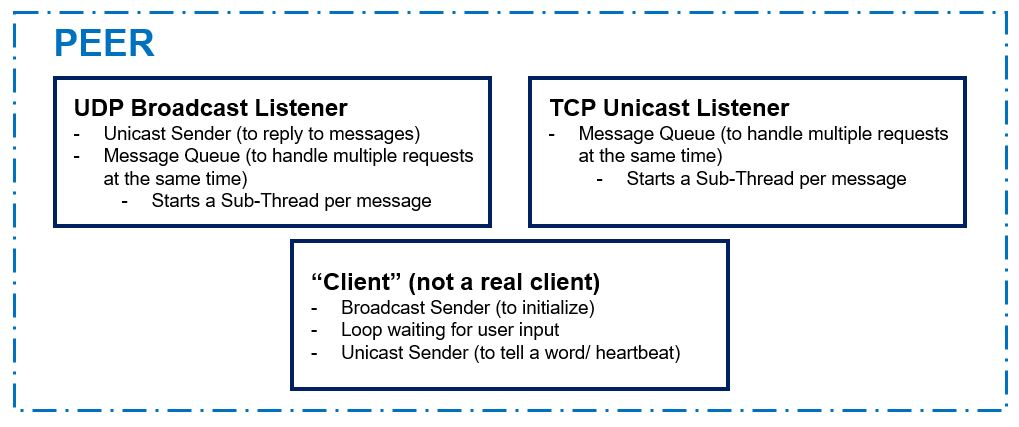
\includegraphics[width=\textwidth]{Peer structure.JPG}
        \caption{Planned structure of peers} \label{fig:peer-structure}
        \end{figure}
        
        Based on a UDP broadcast, each peer then sends a request to join the group. All other peers already on the network respond using TCP unicast with their IP, UUID and group view.  The TCP Unicast listener of the new host receives these messages, sends an acknowledgement to the other peers and can add them to its own group view. To be consistent, the peer then checks the group views and adopts the one that was received the most (Majority must be given). Additionally, each peer can add the new joiner to its own group view. As we consider a topology of an asynchronous uniform non-anonymous ring to be the most suitable for this kind of game, we will implement a logic that allows each peer to find its neighbors.
        
        Figure \ref{fig:dynamic_discovery} shows the sent messages during the dynamic discovery of new peers and how they are added into the own group view of the member.
    
        \begin{figure}[h]
            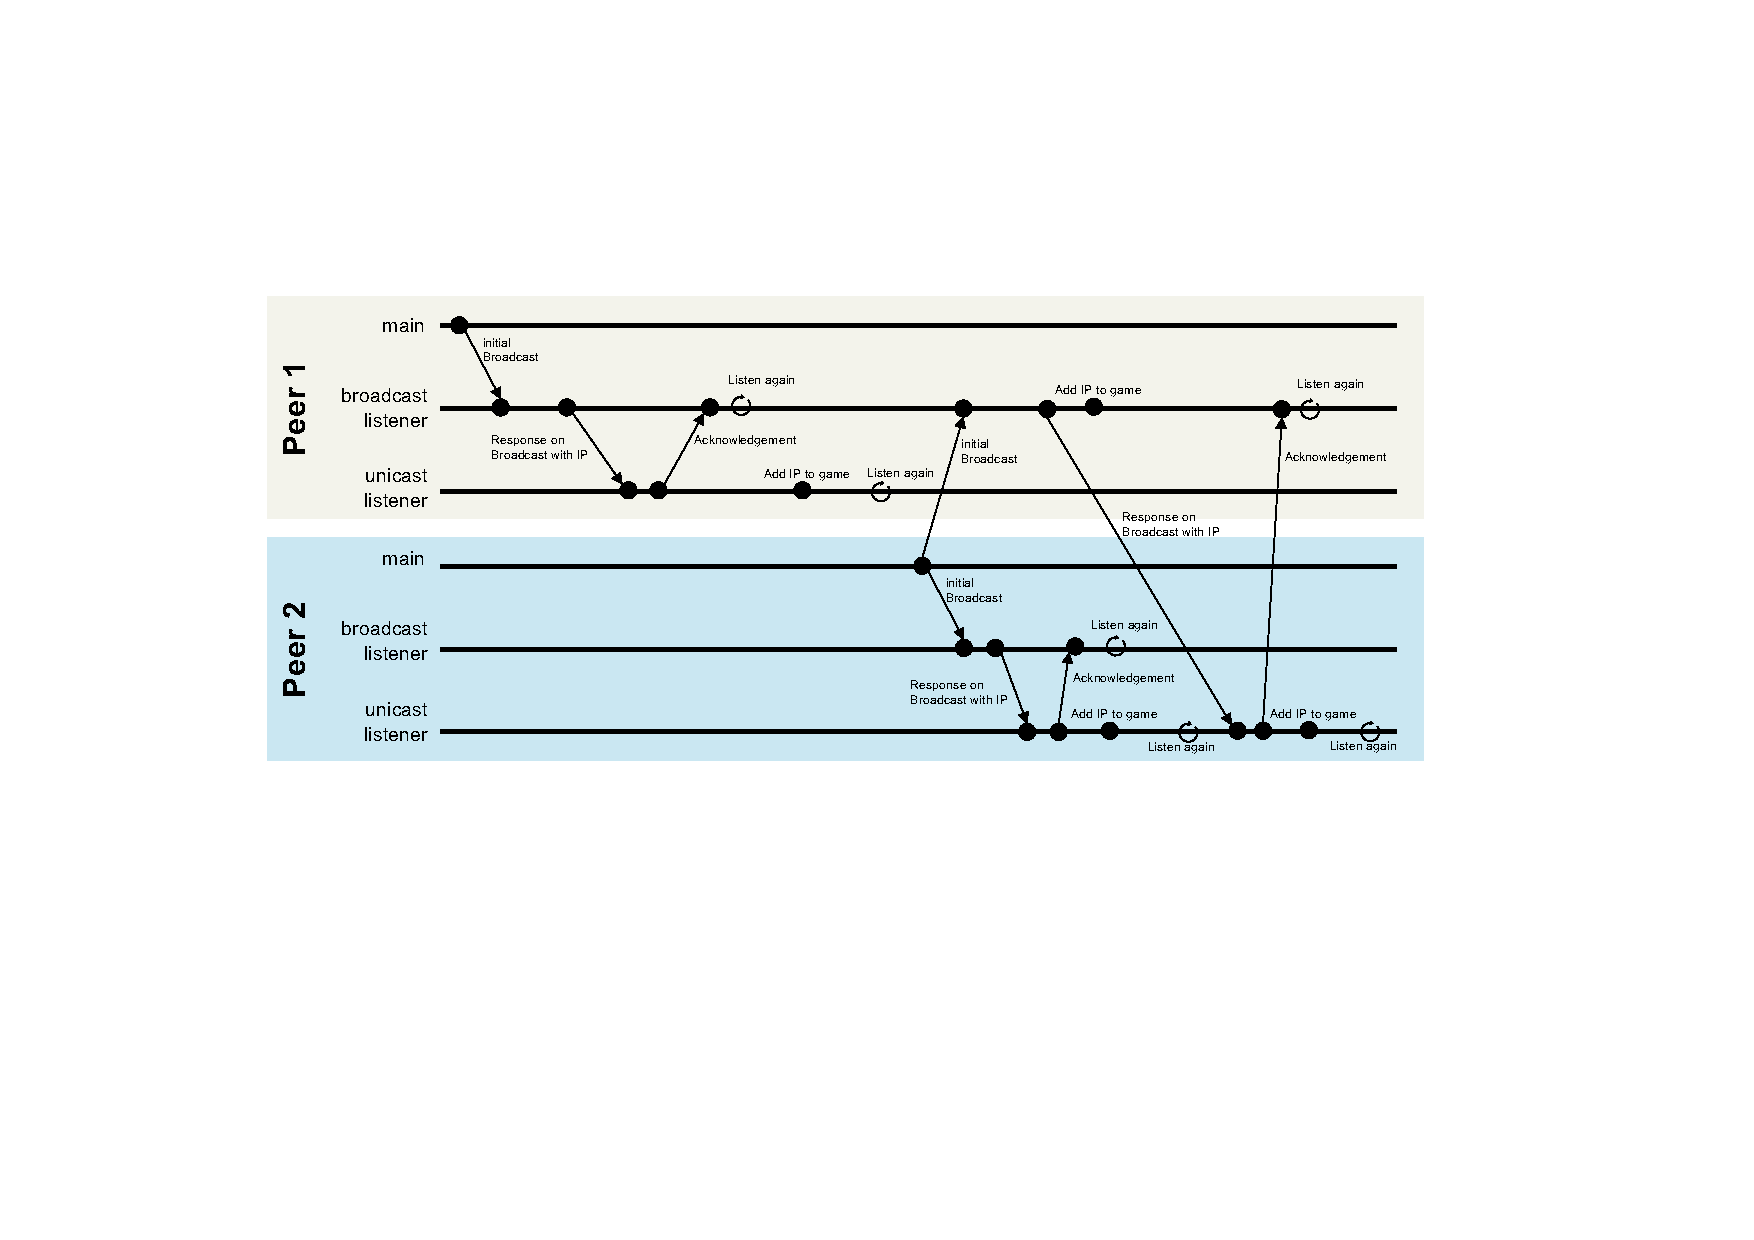
\includegraphics[width=\textwidth]{dynamic_dicovery.pdf}
            \caption{Dynamic Discovery} \label{fig:dynamic_discovery}
        \end{figure}
        
        Once enough peers were detected in the game, the members get the option to initiate a start signal by sending a multicast message to all peers in their group view. Then the system votes and elects a leader and starts the game.
        \\\\
        \textbf{Current implementation state:} We are working on enabling the dynamic discovery of hosts of multiple peers in the same session. At the moment there are still a few problems (see chapter \ref{challenges}). Currently we are in the process of solving them.
        
    \subsection{Crash fault tolerance}
        To ensure that the game is still working once one of the peers crashes, the system must implement crash fault tolerance. Therefore, each peer receives signals from its two neighbors in the ring topology called heartbeats. Those heartbeat messages will be sent through an TCP Unicast. Once a heartbeat is missing, the peer can report the absence to rearrange the topology. In most cases, the rearrangement of the ring should be enough.
        
        But if the current active player crashed during deciding which word to forward, the previous player has to recognize that the crashed active peer was his subsequent neighbour. Now he needs to send his own word again thorough an TCP Unicast to his new following neighbour to allow him to continue.
        
        To ensure the game to continue once the game leader crashed, the system additionally requires the leader to distribute the current game state through an UDP Broadcast with TCP Unicast acknowledgements after each round. If the number of peers falls below the minimum number of three, the system terminates the game and offers the option to start a new one with enough players.
        \\\\
      \textbf{Current implementation state:} Not implemented yet. We are still working on the dynamic discovery of hosts.
        
        %%Additionally, the leader distributes the current game state through an UDP Broadcast after each round. This ensures the continuation of the game if the leader crashes. If the number of peers falls below the minimum number of four, the system waits for new participants to continue.
    
    \subsection{Voting}
        The system must enable initial voting. From this voting a leader emerges, who distributes the points in the game and selects the word from a given list.
        
        In addition, the system must be able to initialize a new voting in case of failure of a peer (if it was the leader) and thus determine a new leader.
    
        When a new peer joins an existing network, the system also checks whether it becomes the new leader.
        
        As we are working in a ring topology, we plan to make use of the LaLann-Chang-Roberts algorithm for the leader election. In this algorithm each peer sends a Unicast message to its neighbour with the next higher UUID. If the arriving UUID is higher then the own, each peer forwards the message in the following step again to its neighbor. If not, the peer drops the message. This way only one message goes through the whole ring and ends up at its initial sender with the same UUID. Once this peer receives its own message, it knows, that it is the elected leader and unicasts the election acknowledgement to its neighbour who forwards it until every peer in the group knows the leader.
        \\\\
        \textbf{Current implementation state:} Not implemented yet. We are still working on the dynamic discovery of hosts.
        
\section{Current Challenges and Blockers}\label{challenges}
    Setting up the system with multiple virtual machines accessing the same network and being able to communicate was a little challenge for some team members that blocked the development in the project some time. At some point we decided to use a work around for those team members to use two physical machines using the same network. Either with this setup or by using multiple virtual machines, the whole team is now able to develop and test the project code.
    \\\\
    When starting into the development, we first setup and tested the basic game logic of whispering words including potential slight changes using a random number. In a next step, we decided to build up the middleware that makes use of some basic functionalities like sockets in python. Here we started with developing the dynamic discovery of participating hosts before initiating the game session. Currently we are facing several challenges regarding the dynamic discovery:
    
    \begin{figure}[h]
        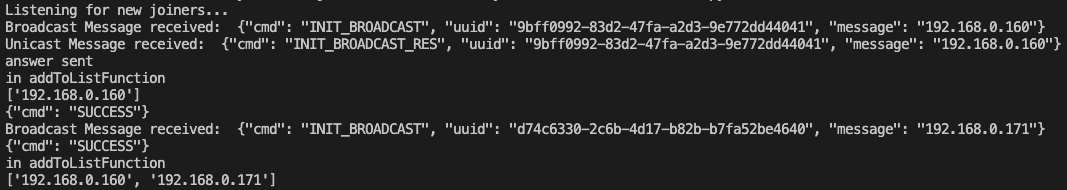
\includegraphics[width=\textwidth]{Dynamic_Discovery_Output.png}
        \caption{Successful detection of two peers} \label{fig:dynamic_discovery_output}
    \end{figure}
    
    \begin{itemize}[label=$\bullet$]
    
    \item  The dynamic discovery currently works well for some machines. This case is shown in Figure \ref{fig:dynamic_discovery_output}. On other machines, the implementation does not work fully correct although the run-time is based on the same code. We noticed that this failure occurs depending on which machine is starting as first peer and which host is joining as second peer. At the moment, our idea is that this failure could be related to some blocking mechanisms in the network.\\
    
    \item We are also wondering whether we need to initiate multiple listeners for Unicast and Broadcast messages in more threads to allow multiple peers to join at nearly the same time. A better way would be to use a queue that stores requests according to the FIFO (fist in - first out) principle. Therefore, listener must create a message queue and start a subthread for each request. This conceptual challenge will intensify later during the project once it comes to receiving heartbeats to allow fault tolerance and the option for peers to join during a running game.\\
    
    \end{itemize}

\end{document}